\chapter{Ausgabemethoden}
\label{cha:Ausgabe}

Im Kapitel~\ref{cha:Eingabe} wurden alternative Eingabemethoden zur Interaktion Hands-Free näher erläutert. Dieses Kapitel befasst sich mit Ausgabemethoden, die aber nicht zwingend an bestimmte Eingabemethoden gebunden sind. So gibt es nicht nur bei Systemen, die beispielsweise über die Sprache gesteuert werden, ein akustisches Feedback, sondern auch bei Systemen, die beispielsweise über die Augen oder den Mund gesteuert werden. 


%%%%%%%%%%%%%%%%%%%%%%% Auditiv %%%%%%%%%%%%%%%%%%%%%%%%%%%
\section{Auditive Ausgabe}

Eine mögliche Form, wie ein Computer ein Feedback geben kann, geschieht durch eine auditive Ausgabe. Dies kann entweder durch ein Geräusch, ein Signal oder durch Sprachausgabe funktionieren.
\newline \newline
Eine Möglichkeit auditives Feedback zu erhalten sind vom Computer erzeugte Signale oder bestimmte Geräusche. Bei diesen Signalen bzw. Geräuschen handelt es sich beispielsweise um einen hohen angenehmen Ton bei korrektem Verhalten oder um einen dumpfen unangenehmen Ton bei einer Fehlereingabe. Darüber hinaus können auch Klick-Geräusche als Ausgabe fungieren. So gibt ein Lautsprecher bei einer Fußgängerampel beispielsweise ein kontinuierliches Klick-Geräusch von sich, wenn es rot ist. Schaltet die Ampel auf grün verdoppeltet sich die Geschwindigkeit des Geräusches.
\newline \newline
Weitaus komplexer funktioniert allerdings die Sprachausgabe. Während bei der Spracheingabe die gesprochene Sprache von einem System in einen Befehl umgewandelt wird, gibt bei der Sprachausgabe der Computer die Informationen in Form von Sprache wieder. Da die Sprachausgabe von Menschen gehört und automatisch bewertet wird, ist es wichtig, dass die Sprache eine hohe Qualität aufweist, also möglichst real erscheint. 
\begin{figure}
\centering
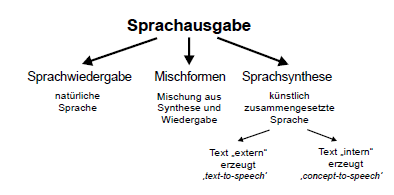
\includegraphics[width=.7\textwidth]{sprachausgabe_overview}
\caption{Unterteilung der Sprachausgabe \cite{FellbaumSprache}.}
\label{fig:SprachausgabeOverview}
\end{figure}
\newline \newline
Wie in Abb.~\ref{fig:SprachausgabeOverview} dargestellt gibt es zwei unterschiedliche Ansätze, wie der Computer den Text in Sprache umwandeln kann:
\begin{itemize}
      \item Sprachwiedergabe
      \item Sprachsynthese
\end{itemize}
\vspace{\baselineskip} \vspace{\baselineskip}
%SPRACHWIEDERGABE
Bei der Sprachwiedergabe werden Sprachsignale ausgegeben, die zuvor aufgenommen und abgespeichert worden sind. Der Umfang an möglichen akustischen Meldungen, also an Wörtern, ist aus diesem Grund an die Anzahl der Aufnahmen gebunden und daher begrenzt. Da die Signale bzw. Wörter von einer realen Person eingesprochen wurden, weist diese Methode eine sehr hohe Sprachqualität auf \cite{KaufmannPfisterSprache}.
\newline \newline
Es gibt unterschiedliche Methoden bzw. Verfahren, wie die Sprachwiedergabe im Detail funktioniert. Zusammenfassend werden die Wörter zu Beginn von einer Person eingesprochen, bearbeitet und abgespeichert. Die einzelnen Sprachelemente werden anschließend adressiert, sodass sie vom System später leicht gefunden werden können. Wenn der Computer nun einen Text vorlesen soll, werden im System anhand der gespeicherten Adressen die einzelnen Wörter bzw. Phrasen herausgesucht und verwendet \cite{FellbaumSprache}.
\newline \newline
%SPRACHSYNTHESE
Im Gegensatz zur Sprachwiedergabe wird bei der Sprachsynthese das Ziel verfolgt, alle möglichen Wortkombinationen in ein Sprachsignal umwandeln zu können. Da die die Wörter, die als Grundlage für die Ausgabe dienen, nicht von einer Person eingesprochen werden, sondern die einzelnen Wörter mit ihrer Betonung künstlich erzeugt werden müssen, sinkt die Sprachqualität und das Endergebnis gleicht oft mehr einer Computerstimme als einer menschlichen. 
\newline \newline
Bei der Sprachsynthese werden Silben aus verschiedenen Wörtern einzeln abgespeichert und so alle beliebigen Kombinationen zusammengesetzt. Im Anschluss werden Betonungen, Lautstärke und Geschwindigkeit hinzugefügt bzw. angepasst. Bei der sogenannten textgesteuerte Sprachsynthese (text-to-speech) ist dem System der eigentliche Inhalt des Textes nicht bekannt. Nicht nur einzelne Sätze bzw. ganze Texte können verarbeitet, sondern auch Konzepte können vom System in Signale umgewandelt werden (concept-to-speech). Das System kreiert einen eigenständigen Text, wenn das Konzept bzw. der Inhalt bekannt ist \cite{FellbaumSprache}.
\newline \newline
%zitat Fellbaum
Laut Fellbaum \cite{FellbaumSprache} besteht die größte Herausforderung der Sprachsynthese darin, die Stimme noch natürlicher und nicht roboterähnlich wirken zu lassen. In der Praxis sind daher Mischformen zwischen Sprachwiedergabe und Sprachsynthese üblich. 


%%%%%%%%%%%%%%%%%%%%%%% Haptisch %%%%%%%%%%%%%%%%%%%%%%%%%%%
\section{Haptische Ausgabe}
%TODO what to write here
%definition haptik
Haptische Ausgabe beinhaltet jenes Feedback, bei dem etwas durch den menschlichen Tastsinn wahrgenommen werden kann. Hierbei gibt es verschiedene Arten:
%
%
\begin{itemize}
      \item Thermales Feedback (Wärme)
      \item Vibration
			\item Feedback durch ein haptisches Steuerungselement
\end{itemize}
\vspace{\baselineskip}
%
%
Bei einer thermalen Ausgabe handelt es sich um ein Feedback in Form von Wärme. Der Computer bzw. das Gerät, mit dem interagiert wird, erhitzt sich auf eine vordefinierte Temperatur und kühlt sich wieder ab. Lee \& Lim \cite{LeeLim} stellten fest, dass warme Temperaturen mit etwas Positivem und kalte Temperaturen mit etwas Negativem verbunden werden. Des Weiteren konnten die Teilnehmer Abstufungen der Wärmeunterschiede wahrnehmen, die eine strikte Trennung von warm oder kalt überschreiten. Die Veränderungen von warm auf kalt oder umgekehrt sollen nicht zu plötzlich geschehen, da dies ein Unwohlbefinden bei der Interaktion auslöst \cite{LeeLim}. \newline
Laut Jones & Berri \cite{JonesBerris} soll sich das Ausgabegeräte um höchstens 20°C pro Sekunde abkühlen und um max. 10°C pro Sekunde aufwärmen. Die Spanne der Temperatur sollte sich im Bereich zwischen 5°C und 45° befinden, da dieser Bereich am besten von den Rezeptoren in der Haut wahrgenommen werden kann.
\newline \newline
Eine haptische Ausgabe ist auch in Form von Vibration möglich. Die Vibration unterscheidet sich in ihrer Intensität und Dauer. Diese Art von Feedback kann unter anderem zur Bestätigung einer Eingabe erfolgen \cite{Vibration}. Will ein Benutzer beispielsweise auf einer virtuellen Tastatur einen Buchstaben auswählen, wird bei Erfolg eine leichte Vibration durch ein Armband o.ä. erfolgen.
\newline \newline
%% TODO Haptisches Stuerelement%%
Neben der thermalen Ausgabe und der Ausgabe durch Vibration ist das Feedback auch über das Eingabeelement möglich. Handelt es sich bei dem Eingabegerät um einen Joystick, kann die Ausgabe durch verschiedene Vibrationsmuster, aber auch durch eine Gegenbewegung des Joysticks in X-, Y- oder Z-Richtung erfolgen, je nachdem wie viele Freiheitsgrade das Eingabegerät erlaubt (vgl. Abschnitt ~\ref{cha:Kinnsteuerung}) \cite{an2002haptic}. 
\newline \newline
Es gibt unterschiedliche Möglichkeiten, wie haptische Ausgabe geschehen kann. Soll eine Eingabe besätigt werden, ist ein Feedback zu Vibration meist üblich. Soll ein möglichst realistisches Feedback bzw. eine Interaktion mit dem System gewährleistet werden, ist darüber hinaus ein Feedback vom Eingabeelement durch Bewegungsrichtung empfehlenswert.  
\newpage
%%%%%%%%%%%%%%%%%%%%%%% Visuell %%%%%%%%%%%%%%%%%%%%%%%%%%%
\section{Visuelle Ausgabe}
%TODO what to write here
Um Informationen visuell darzustellen und diese als Ausgabe des Systems zu nutzten, sind ein oder mehrere Displays oder Projektoren notwendig. Die Ausgabe kann entweder auf dem selben Bildschirm wie die Eingabe zu sehen sein, oder auf einem separaten Bildschirm.
\newline \newline
Es gibt sehr viele unterschiedliche Formen und Ausprägungen, wie eine visuelle Ausgabe erfolgen kann. Dies beginnt bei der simplen Ausgabe eines Textes. Wird eine bestimmte Interaktion richtig oder falsch ausgeführt, kann daraufhin ein Text bzw. ein Wort erscheinen, das den Erfolg bzw. Misserfolg mitteilt. Des Weiteren können auch Bilder oder andere Mediaelemente in einem ähnlichen Kontext gezeigt. Bei der bloßen Unterscheidung zwischen korrekt und inkorrekt erscheint beispielsweise ein grünes Häkchen bzw. rotes Kreuz. Visuelle Ausgabe erfolgt aber nicht nur über unterschiedliche Symbole, auch die bloße Änderung der Farbe eines Elementes kann ausschlaggebend für dessen Zustand sein.
\newline \newline
Abb.~\ref{fig:MyoTraining}(a) beschreibt einen Kalibrierungsschritt vor der Verwendung eines Systems, das durch die Muskelkontraktionen gesteuert werden kann. Hier gibt der Computer laufend ein visuelles Feedback über den aktuellen Zustand bzw. die Anspannung der Muskeln.
\newline \newline
Bei dem in Abschnitt ~\ref{cha:Augensteuerung} erwähnten Augensteuerungssystem des Unternehmens%
\footnote{http://humanelektronik.de/}
%
kann eine virtuelle Tastatur mit Hilfe der Augen bedient werden. Wird ein Buchstabe über einen längeren Zeitraum fokussiert, wird dieser auch ausgewählt. Während der Fixation erscheint eine Sanduhr, die dem Benutzer mitteilt, wie lange der gewünschte Buchstabe noch fixiert werden muss \cite{SEETECH}. 
%
\newline \newline
Zusammengefasst kann gesagt werden, dass es sehr viele verschiedene Möglichkeiten gibt, wie ein Computer bzw. das Interaktionsgerät selbst visuell Feedback geben kann. Je nach Anwendungsfall, ob es sich beispielsweise um eine richtig oder falsch Unterscheidung oder um eine komplexere Ausgabe handelt, können Texte, Symbole, Farben oder auch Kombinationen ausgewählt werden.
%
%
%abschlussatz
\newline \newline \newline
Alle beschriebenen Ausgabemethoden können einem menschlichen Sinn zugeordnet werden (auditive Ausgabe dem Hörsinn, haptische Ausgabe dem Tastsinn und visuelle Ausgabe dem Sehsinn). 
Erwähnenswert wäre auch, dass es eine Ausgaben gibt, die dem Geschmackssinn und dem Geruchssinn zugeordnet werden können. Allerdings kommen diese in der Praxis nur vereinzelt zum Einsatz und werden daher im Zuge dieser Arbeit nicht vertiefend erläutert.


